% This work is made available under the terms of the
% Creative Commons Attribution-ShareAlike 4.0 license,
% http://creativecommons.org/licenses/by-sa/4.0/.

\documentclass[a4paper]{book}

\usepackage{wrapfig}
\usepackage{graphicx}
\usepackage{hyperref}
\usepackage{multirow}
\usepackage{scalefnt}
\usepackage{tikz}

% watermark -- for draft stage
%\usepackage[firstpage]{draftwatermark}
%\SetWatermarkLightness{0.9}
%\SetWatermarkScale{5}

% Copyright (c) 2009 by the University of Waikato, Hamilton, NZ. 
% This work is made available under the terms of the 
% Creative Commons Attribution-ShareAlike 4.0 license,
% http://creativecommons.org/licenses/by-sa/4.0/.
%
% Version: $Revision: 5479 $

\newenvironment{tight_itemize}{
\begin{itemize}
  \setlength{\itemsep}{1pt}
  \setlength{\parskip}{0pt}
  \setlength{\parsep}{0pt}}{\end{itemize}
}

\newenvironment{tight_enumerate}{
\begin{enumerate}
  \setlength{\itemsep}{1pt}
  \setlength{\parskip}{0pt}
  \setlength{\parsep}{0pt}}{\end{enumerate}
}

% if you just need a simple heading
% Usage:
%   \heading{the text of the heading}
\newcommand{\heading}[1]{
  \vspace{0.3cm} \noindent \textbf{#1} \newline
}

\newcommand{\icon}[1]{\tikz[baseline=-3pt]\node[inner sep=0pt,outer sep=0pt]{\includegraphics[height=1.1em]{#1}};}


\title{
  \textbf{ADAMS} \\
  {\Large \textbf{A}dvanced \textbf{D}ata mining \textbf{A}nd \textbf{M}achine
  learning \textbf{S}ystem} \\
  {\Large Module: adams-tensorflow} \\
  \vspace{1cm}
  
\includegraphics[width=2cm]{images/tensorflow-module.png} \\
}
\author{
  Peter Reutemann
}

\setcounter{secnumdepth}{3}
\setcounter{tocdepth}{3}

\begin{document}

\begin{titlepage}
\maketitle

\thispagestyle{empty}
\center
\begin{table}[b]
	\begin{tabular}{c l l}
		\parbox[c][2cm]{2cm}{\copyright 2018-2019} &
		\parbox[c][2cm]{5cm}{
\includegraphics[width=5cm]{images/coat_of_arms.pdf}} \\
	\end{tabular}
	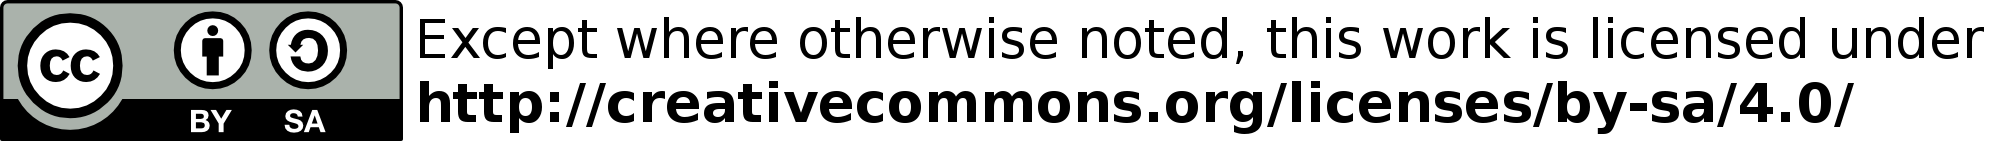
\includegraphics[width=12cm]{images/cc.png} \\
\end{table}

\end{titlepage}

\tableofcontents
%\listoffigures
%\listoftables

%%%%%%%%%%%%%%%%%%%%%%%%%%%%%%%%%%%
\chapter{TensorFlow}
TensorFlow\cite{tensorflow} is an open source software library for high performance
numerical computation. Its flexible architecture allows easy deployment of
computation across a variety of platforms (CPUs, GPUs, TPUs), and from desktops
to clusters of servers to mobile and edge devices. Originally developed by
researchers and engineers from the Google Brain team within Google's AI
organization, it comes with strong support for machine learning and deep
learning and the flexible numerical computation core is used across many other
scientific domains.


%%%%%%%%%%%%%%%%%%%%%%%%%%%%%%%%%%%
\chapter{Flow}
In order to use Tensorflow's Object Detection API\cite{objdet}, it is necessary
to create tfrecords\cite{tfrecord} from your annotated data.
Generating the tfrecords can be achieved with the \textit{wai.tfrecords}\cite{waitfrecords}
library. But rather than having to split the data manually in train and test sets,
you can use ADAMS' functionality to separate file lists into subsests (e.g., using
\textit{PrepareFileBasedDataset}).

To set up the wai.tfrecords library, create a virtual environment (Python 3.7+)
and install the requirements from \textit{adams-tensorflow-generate\_tfrecords-requirements.txt}.

\noindent For instance, on Linux run these commands (adjust the path accordingly):
{\scriptsize
\begin{verbatim}
virtualenv -p /usr/bin/python3.7 venv
./venv/bin/pip install -r adams-tensorflow-generate_tfrecords-requirements.txt
\end{verbatim}}

\noindent With the virtual environment in place, you can run the following flows:
\begin{tight_itemize}
  \item \textit{adams-tensorflow-generate\_tfrecords-cv.flow} -- generates cross-validation folds
  \item \textit{adams-tensorflow-generate\_tfrecords-split.flow} -- generates train/test split
\end{tight_itemize}
When prompted by the flows to supply a Python executable, simply select the
executable from within the previously generated virtual environment. The flow
will construct file lists from the input data and call the conversion script
to generate tfrecord files (and label/file lists) from these.


%%%%%%%%%%%%%%%%%%%%%%%%%%%%%%%%%%%
% Copyright (c) 2009-2012 by the University of Waikato, Hamilton, NZ. 
% This work is made available under the terms of the 
% Creative Commons Attribution-ShareAlike 4.0 license,
% http://creativecommons.org/licenses/by-sa/4.0/.
%
% Version: $Revision$

\begin{thebibliography}{999}
	% to make the bibliography appear in the TOC
	\addcontentsline{toc}{chapter}{Bibliography}

    % references
	\bibitem{adams}
		\textit{ADAMS} -- Advanced Data mining and Machine learning System \\
		\url{https://adams.cms.waikato.ac.nz/}{}
		
	\bibitem{heatmap}
		\textit{Heat map} -- WikiPedia article \\
		\url{http://en.wikipedia.org/wiki/Heat_map}{}

\end{thebibliography}


\end{document}
